\documentclass{report}
\usepackage[T1]{fontenc}
\usepackage[utf8]{inputenc}
\usepackage{lmodern}
\usepackage[numbers]{natbib}
\usepackage{amsthm}
\usepackage{amsmath}
\usepackage{graphicx}
\usepackage{float}
\usepackage{capt-of}
\usepackage{subfigure}
\usepackage{listings} 
\usepackage{cases}
\usepackage{comment}
\usepackage{mathtools}
\usepackage{enumitem}


\title{Stock Market Prediction}
\author{Mark Dunne}

\begin{document}

\lstset{language=Python}    
\belowdisplayskip=12pt plus 3pt minus 9pt
\belowdisplayshortskip=7pt plus 3pt minus 4pt

\maketitle

\begin{abstract}

In this report we analyse existing and new methods of stock market prediction. We take three different approaches at the problem: Fundamental analysis, Technical Analysis, and the application of Machine Learning. We find evidence in support of the weak form of the Efficient Market Hypothesis, that the historic price does not contain useful information but out of sample data may be predictive. We show that Fundamental Analysis and Machine Learning could be used to guide an investor's decisions. We demonstrate a common flaw in the Technical Analysis methodology and show that it produces limited useful information. Based on our findings, an algorithmic trading program is developed and entered into the Quantopian trading competition.

\end{abstract}

\tableofcontents

\chapter{Introduction}

Predicting the Stock Market has been the goal and bane of investors since its existence. Everyday billions of dollars are traded on the exchange, and behind each dollar is an investor hoping to profit in one way or another from their predictions. Entire companies rise and fall daily based on the behaviour of the market. Should one be able to accurately predict market movements, it offers a tantalizing promises of wealth and influence. 

It is no wonder then that the Stock Market and its associated difficulties find their way into the public imagination every time it misbehaves. The 2008 financial crisis was no different as evidenced by the flood of films and documentaries on the topic. If there was a common theme among those productions, it was that no one was really sure how the market works and reacts. Perhaps a better understanding of stock market prediction might help in the case of similar events in the future.

\section{Project Goals and Scope}

Dispite its prevalence, Stock Market prediction remains a secretive and empiracal art. Few people, if any, are willing to share what  successful strategies they may have. A chief goal of this project is to add to the academic understanding of stock market prediction. The hope is that with a greater understanding of how the market moves, investors will be better equiped to prevent another financial crisis. The project will evaluate some existing strategies from a rigorous scientific perspective and provide a quantitative evaluation of new strategies. 

It is also important here to define the scope of the project. Although vital to any investor operating in the real world, no attempt is made in this project at portfolio management. Portfolio management is largely an extra step done after an investor has made a prediction on which direction any particular stock will move. The investor may choose to allocate funds across a range of stocks in such a way to minimize his or her risk. For instance, the investor may choose not to invest all of their funds into telecoms companies, just in case the entire sector takes an unexpected turn. A more common approach would be for an investor to invest across a broad range of stocks based on some critera he has decided on before. 

This project will focus on predicting the daily movement direction (price going up or down) of individual stocks. The project will make no attempt at deciding how much money to allocate to each prediction.  More so, the project will analyse the accuracies of these predictions. 

\chapter{Data and Tools}

\section{Data Used}

\subsection{Choosing the Dataset}

For this project, we chose the Dow Jones and its components as a representative bundle of stocks. The Dow Jones is a large index traded on the New York stock exchange. It is a price-weighted index over 30 component companies [todo show calculation]. All companies in the index are large publicly traded companies, leaders in each of their own sectors. The index covers a diverse set of sectors featuring companies such as Microsoft, Visa, Boeing, and Walt Disney.

It is important to use a predefinied set of companies instead of a custom selected set so that we do leave ourselves open to methodology errors or accusations of fishing expeditions. If we had selected a custom set of companies, it could be argued that the set was taylored specifically to improve our results. Since the aim of the project is to create a predictive model of stock markets in general, this is a claim that we want to avoid. 

The Dow Jones was chosen because it is well known, and has a relatively small number of compontents. The leading index, the S\&P 500 has over 500 components, but ultimately analysing 500 companies proved to be too computationally expensive for the resources at hand. This small but representitiive set of 30 components allowed for a managable dataset given limited resources. Although there were only 30 companies, there was no lack of data to study. To test many of the hypotheses laid out in this report, we were able to extract datasets many thousands of examples in size.

\subsection{Gathering the Datasets}

Luckily, data on daily stock prices is easy to come by. Google and Yahoo both operate websites which offer a facility to download CSV files containing a full daily price history. These are useful for looking at individual companies but are slightly cumbersome to use when analysing large amounts of data. 

Instead of using Google and Yahoo directly, Quandl\cite{website:quandl} was used to gather the data. Quandl is a free to use website that hosts and maintains vast amounts of numerical datasets with a focus specifically on economic datasets. It also provides a small python library that is useful for accessing the database programmatically. The library also provides a simple method for calculating the daily percentage change in prices. This calculation is defined in equation \ref{eq:quandl-pc-calc} where $p_{t}$ is the closing price on day $d$, and $\delta p_{d}$ is the resulting percentage change.  

\begin{figure}[H]
\begin{center}
    \begin{equation}
      \delta p_{d} = \dfrac{p_{d} - p_{d-1}} {p_{d-1}}
      \label{eq:quandl-pc-calc}
    \end{equation}
\end{center}
\end{figure}

To build the primary dataset, a simple program was built to query the Quandl API for each of the 30 Dow Jones components using the transformation outlined in equation \ref{eq:quandl-pc-calc}. Before finally saving the data, the gathered data was augmented with an additional column containing the classificiation of the daily percentage change. This augmentation is defined in equation \ref{eq:quandl-pc-class} where $trend_{d}$ is the price movement direction on day $d$ and $\delta p_{d}$ as defined in equation \ref{eq:quandl-pc-calc}.

\begin{figure}[H]
\begin{center}
\begin{equation}
trend_{d} = \begin{cases}
Loss &\text{if $\delta p_{d} < 0$}\\
Gain &\text{if $\delta p_{d} > 0$}\\
Neutral &\text{if $\delta p_{d} = 0$}
\end{cases}
\label{eq:quandl-pc-class}
\end{equation}
\end{center}
\end{figure}

The final step is shifting all of the $\delta p_{d}$ and $trend_{d}$ data points backwards by one day. This is done because these are the dependent variables that we are trying to predict. The data we have for any day should be used to predict the trend tomorrow, not the same day. By doing this, data in later sections we gather for a Monday will be matched with the Tuesday's trend.

This dataset was then saved in CSV format for simple retrival as needed throughout the project. This dataset containing the daily trends of companies will serve as the core dataset that will be used in most experiments later in the report. When we want to use the dataset later with the extra data we collect for each experiment, we only need to do a simple database join operation on the company and date. The dataset contains 122,121 rows covering all 30 companies daily since January 1st 2000. Table \ref{table:data-example-0} shows an extract of the number of rows from this dataset.

\begin{figure}[H]
\caption{Data Extract of Primary Dataset}
\begin{center}
  
    \begin{tabular}{l | l | l | l }
      Date & Symbol & $\delta p_{d}$ & trend \\ \hline
      2000-01-05 & DD  &	0.04230 	& Gain \\ \hline
      2000-01-05 & DIS &	0.03748 	& Gain \\ \hline
      2000-01-05 & GE  &	-0.00749 	& Loss \\ \hline
      2000-01-05 & GS  &	-0.04248 	& Loss \\ \hline
      2000-01-05 & HD  &	-0.00097 	& Loss \\ \hline
      2000-01-05 & IBM &	0.03515 	& Gain

    \label{table:data-example-0}
    \end{tabular}
\end{center}
\end{figure}

With the primary dataset prepared, we will combine it as needed with additional datasets to carry out individual experiments. 

\subsection{Limitations of the Data}

Although the data gathered in the previous section is certainly a good start, it is admittedly far behind what any serious investor more than likely has access to. An obvious side of the data that is missing is the intraday prices, i.e the prices minute by minute. It is possible that this data could be used to guide and investors decisions on the interday level. However, intraday prices are not as freely available as interday prices and are considered a commodity in themselves. To get hold of such a dataset would incur a large cost, one that is not in the budget of a project such as this. Later in the project we will evaluate a strategy in which this limitation becomes significant.

Another important piece of the data puzzle that the project is missing is the order book. The order book is a record of buy and sell orders of each particular stock. It consists of the amount a trader is willing to buy and sell, as well as their price. Successful orders are matched off against the order book by the exchange. The actual price of a stock is usually considered to be half way between the highest buying price and the lowest selling price. It is easy to imagine that the order book contains useful data. For instance, the weighted average price of all orders on the order book might be predictive of the actual price. However access to this data is extremely costly and far beyond what most casual investors can afford, let alone this project's budget.

With no way around these limitations, we do our best with the data that Quandl provides.

\section{Tools}
\subsubsection{Python and associated packages}

Python was the language of choice for this project. This was an easy decision for the following reasons.

\begin{enumerate}
  \item Python as a language has an enourmous community behind it. Any problems that might be encountered on the way can be easily solved with a trip to Stack Overflow. Python is among the most popular languages on the site which makes it very likely there will be a direct answer to any query \cite{website:redmonk-languages}. 
  
  \item Python has an abundance of powerful tools ready for scientific computing. Packages such as Numpy, Pandas, and SciPy are freely available, performant and well documented. Packages such as these can dramatically reduce and simplify the code needed to write a given program. This makes iteration quick.

  \item Python as a language is forgiving and allows for programs that look like pseudo code. This is useful when pseudo code given in academic papers needs to be implemented and tested. Using Python, this step is usually reasonably trivial.

\end{enumerate}

However, Python is not without its flaws. The language is dynamically typed and packages are notorious for Duck Typing. This can be frustrating when a package method returns something that, for example, looks like an array rather than being an actual array. Coupled with the fact that standard Python documentation does not explicitly state the return type of a method, this can lead to a lot of trial and error type testing that would not otherwise happen in a strongly typed language such as Haskell. In my view, this is an issue that makes learning to use a new Python package more difficult than it otherwise could be.

\chapter{Considerations in Approaching the Problem}

Throughout the project, there are three ideas that warn us that we might not actually find a profitable way to predict market trends.

\section{Random Walk Hypothesis}

The random walk hypothesis sets out the bleakest view of the predictibility of the stock market. The hypothesis says that the market price of a stock is essentially random. The hypothesis implies that any attempt to predict the stock market will inevitably fail. 

The term was popularized by \citet{malkiel1999random}. Famously, he demonstrated that he was able to fool a stock market 'expert' into forecasting a fake market. He set up an experiment where he repeatedly tossed a coin. If the coin showed heads, he moved the price of a fictitious stock up, and if it showed tails then he moved it lower. He then took his random stock price chart to a supposed expert in stock forecasting, and asked for a prediction. The expert was fooled and recommended that he buy the stock immediately. 

It is important for the purpose of this project to confront the Random Walk Hypothesis. If the market is truely random, there is little point in continuing. 

\subsection{Qualitative Similarity to Random pattern}

The stock market can certainly look random to the eye of a casual observer. To demonstrate this, we generated a random process with similar visual characteristics to the Dow Jones index.

We created a perfectly random process that had striking visual similarity to real stock market data using the following simple formula.

\begin{align*}
	a_{x} = a_{x-1} * \rho + q_{x}\\
	b_{x} = b_{x-1} + \rho * r_{x}\\
	f(x) = a_{x} + b_{x}\\
\end{align*}

For the best results, $\rho$ was given a value between 0.995 and 1, while $q$ and $r$ are random values taken from a standard normal distribution. 

\begin{figure}[H]
	\caption{Example of random pattern generated}
	\centerline{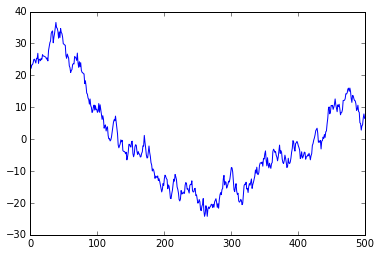
\includegraphics[width=\textwidth]{vis/random-process.png}}
	\label{fig:random-process}
\end{figure}

We then compare this random process to a real piece of market data.

\begin{figure}[H]
	\caption{Centered APPL stock price, some time after 2010}
	\centerline{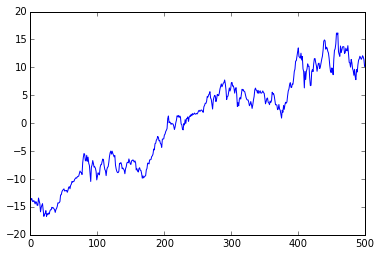
\includegraphics[width=\textwidth]{vis/appl.png}}
	\label{fig:appl-process}
\end{figure}

Presented with both of these diagrams, and without the aid of time scales or actual prices, most people would find it impossible to differentiate the diagrams. Using visual inspection alone, either of these diagrams could just as likely be a real piece of stock market data.

This gives us pause as there is little point in moving forward if the stock market is truly random and there is nothing to predict. However, this does not turn out to be the case. We will demonstrate that it is different to random in two ways. In the very next section, we will show that the price itself is fundamentally different to random data, and later we will show that the price is not as random as it may appear when we take external variables into account.

\subsection{Quantitative Difference to Random pattern}

We will first show that the way in which markets move is fundamentally different to the way one would expect them to move if they were random.

\citet{karpio2007gain} describe an asymmetry between gains and losses on the stock market. Their research looks specifically at indices like the Dow Jones and how "you wait shorter time (on average) for loss of a given value than for gain of the same amount". However, this research was conducted in 2006, before the Great Recession. It is conceivable that the market conducts itself differently since then, and therefore we tried to replicate their findings.

On every day from the year 2000 to 2014, we simulated an investment on the Dow Jones index. We then counted the number of days it took for the investment to gain or lose 5\% of its original value. When it lost 5\% of its value, it was put into the red set, when it gained 5\% of its original value, it was put into the green set. The graph shows two overlaid histograms detailing how long it took for an investment to lose or gain 5\%.

\begin{figure}[H]
	\caption{Gain-Loss Asymmetry on the Dow Jones}
	\centerline{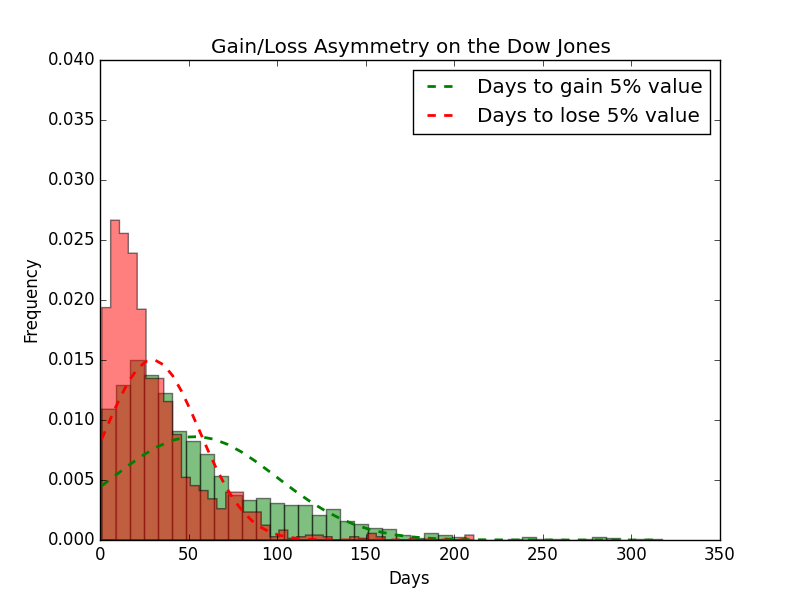
\includegraphics[width=\textwidth]{vis/gain_loss_asymmetry.png}}
	\label{fig:gain-loss-asymm}
\end{figure}

What this graph shows is that the market generally creeps upwards but is prone to sudden drops downwards, and supports the findings described earlier. This demonstrates that the stock market is fundamentally different to random data. This gives us hope for the remainder of the project. If the market price is not random, then it might be worth investigating and trying to predict.

\section{Efficient Market Hypothesis}

Another concept to keep in mind while working on the project was the Efficient Market Hypothesis. Informally, the Efficient Market Hypothesis says that the market is efficient at finding the correct price for the stock market.

It comes in three flavors. However it is still a matter of debate which one, if any, is correct.

\begin{description}
  \item[Weak-form Efficient Market Hypothesis] 
  The weak form of the hypothesis says that no one can profit from the stock market by looking at trends and patterns within the price of a product itself. It is important to note that this does not rule out profiting from predictions of the price of a product based on data external to the price. We will see examples of prediction based on both in sample and out of sample data, and provide evidence in support of the weak form.
  
  \item[Semi-Strong Efficient Market Hypothesis]
  The semi-strong form rules out all methods of prediction, except for insider trading. This means that if we are only to use public domain information in our prediction attempt, the semi-strong form says that we will be unsuccessful. Later in the project, we will provide results that appear to support this hypothesis but not as strong as with the weak form.
  
  \item[Strong form Efficient Market Hypothesis]
  The strong form says that no one can profit from predicting the market, not even insider traders.
\end{description}


Clearly, if we are to predict the stock market using only public information, we must hope that at most the weak form of the Efficient Market Hypothesis is true so that at least then we can use external data to predict the price of a product.

\section{Self Defeating Strategies}

Finally there is the idea of a successful model ultimately leading to its own dimise. 

The insight is that if there were a simple predictive model that anyone could apply and profit from themselves, then over time all of the advantage will be traded and erroded away.

This is the same reason for the lack of academic papers on the topic of successfully predicting the market. If a successful model was made widely known, then it wouldn't take long until it wouldn't be successful any more.

\section{Conclusions}

The three preceding ideas ask us to keep an open mind on stock market prediction. It is possible that we will not be able to do it profitably.

\chapter{Review of Existing Work}

In this section, we will review existing academic literature in regard to predicting the stock market. We will look at two articles, one in support of technical analysis methods and another in support of machine learning methods. We will see that both leave room for improvement.

\section{Article 1 - \citet{kara2011predicting}} 

[todo need to explain technical analysis before this]

The first article we will review is \textit{Predicting direction of stock price index movement using artificial neural networks and support vector machines: The sample of the Istanbul Stock Exchange} by \citet{kara2011predicting}. 

The article makes a case for using technical analysis to predict the direction of the ISE National 100 Index, a stock index traded on the Istanbul Stock Exchange. The article claims impressive results, up to 75.74\% accuracy.

The team uses a set of 10 technical analysis indicators and applies each of them to the price history of the National 100 Index price history. The indicators used are listed below.

\begin{itemize}[noitemsep]
  \item Simple 10-day moving average
  \item Weighted 10-day moving average
  \item Momentum
  \item Stochastic K\%
  \item Stochastic D\%
  \item Relative Strength Index
  \item Moving Average Convergence Divergence
  \item Larry Williams R\%
  \item Accumulation Distribution Oscillator
  \item Commodity Channel Index
\end{itemize}

This data is then coupled with the price movement direction, the dependent variable and used to train two types of model. The models used are a Support vector machine, and a neural network. Results are cross-validated using a single-holdout method. This method of cross-validation is known to be inferior when compared to other techniques such as k-fold cross-validation \cite{kohavi1995study}, but it is unlikely that this would have a drastic effect on the results presented in the article. The team's neural network model had an average performance of 75.74\% accuracy and their support vector machine had an average performance of 71.52\% accuracy.

These results are in sharpe contrast with work that we will present later in the report. The first reason this might be is that prehaps the Istanbul stock exchange is more accommodating to technical analysis than the 30 Dow Jones components reviewed in this report. This is understandable since all 30 of the Dow Jones components are traded on the New York Stock Exchange, which is the most computerised exchange in the world. It is likely that there are less trading algorithms competing on the Istanbul stock exchange and it is therefore easier to leverage algorithmic approaches. 

There is another large flaw however in the methodology of the article that is far more likely to have dramatically increased the performance of their algorithms. In section three of the article, the team describes how they prepared their research data. Specifically, 

\begin{quotation}
\textit{The direction of daily change in the stock price index is categorized
as ‘‘0’’ or ‘‘1’’. If the ISE National 100 Index at time $t$ is higher
than that at time $t-1$, direction $t$ is ‘‘1’’. If the ISE National 100
Index at time t is lower than that at time $t-1$, direction $t$ is ‘‘0’’.}
\end{quotation}

At first this would appear sensible, but their calculations also use the same $t$. For example, their moving average calculation is defined in equation \ref{eq:article1-sma-calc} where $C_{t}$ is the closing price at time $t$.

  \begin{figure}[H]
  \begin{center}
      \begin{equation}
        \text{Simple 10-day moving average} = \dfrac
          {C_{t} + C_{t-1} + ... + C_{t-10}} {10}
        \label{eq:article1-sma-calc}
      \end{equation}
  \end{center}
  \end{figure} 

In \ref{eq:article1-sma-calc}, the simple moving average is calculated using the closing price at time $t$ and $t-1$. In fact all features used in the article use some information from time $t$ and $t-1$, as well as others. But what they were trying to predict is the difference between $t$ and $t-1$. This means, in effect, that they are using information about tomorrow to predict tomorrows price. In a real world situation, no trader or trading algorithm would have the same level of information about tomorrow when they are making their predictions. If we wish to remain true to the idea of stock market prediction, we should only provide our models with information they could have in the world world. Clearly, this is a large flaw in the article. 

However, it can be argued that the work may still be useful. Although the impressive figure of 75.74\% prediction accuracy would be impossible to replicate in a real world model because of the problems described above, perhaps it tells us something else. We could reinterpret the 75.74\% accuracy result not as predictive accuracy, but how accurately the technical analysis indicators agreed reality. In other words, even though the features ultimately had access to the movement direction because of the overlapping times, they agreed with it 75.74\% of the time. 

Using this interpretation, \citet{kara2011predicting} have not demonstrated the predictive power of technical analysis, but demonstrated that it might be worth investigating. Later in this report, we will apply the corrected methodology and attempt to build a model using some of the same features.

\section{Article 2 - \citet{shen2012stock}}

The second article we will look at is \textit{Stock Market Forecasting Using Machine Learning Algorithms} by \citet{shen2012stock}.

The article makes a case for the use of machine learning to predict large american stock indicies, including the Dow Jones. The article boasts a 77.6\% accuracy rate for the Dow Jones specificially. 

The team uses a set of 16 financial products and and uses their movements to predict movements in american stock exchanges. Some of the financial products used are listed below.

\begin{itemize}[noitemsep]
  \item FTSE index price
  \item DAX index price
  \item Oil price
  \item EURO/USD exchange rate
\end{itemize}

The article makes good use of explorative methods in their data preparation stage. They show using graphs there there is a some features may have predictive power because of their correlation to the NASDAQ index. 

They then go on to perform feature selection based on the predictive power of each feature on its own. The results presented in this section, the predictive power of single features, are very similar to results that we will show later in this report. 

After they have selected their top 4 features they compare a Support vector machine model to a Multiple Additive Regression Trees model for predicting the following day's NASDAQ trend. Their winning model is the SVM with 74.4\% accuracy. 

While the results presented by \citet{shen2012stock} in this article appear to be very much inline with results that will be later presented in this report, it is quite vague in terms of the methodology that was used. For instance, there is no record of what model was used in the feature selection step or how cross-validation was carried out to calculate any of their results. However because their results will be supported by ours, we don't imagine that any critical errors were made in these steps.

After they successfully train and test a model, they use it to simulate a real life trading environment. Their models perform extremely well on the simulated trading example with an average of an 8\% return rate every 50 days. This is where the results of this article and the results of our report diverge. This article fails to account for overlapping trading hours. For instance the FTSE, which is traded in London, and the Dow Jones, which is traded in New York, are both trading simultaneously for three to four hours each day. This is enough time for the New York stock exchange to influence the London Stock stock exchange. It follows then that it is incorrect to use the closing prices in London to predict New York's movements.

While training and testing the models, both the article and this report ignore the overlapping of trading hours. However, this should certainly not be ignored when simulating real world trading. Later in this report, we will simulate real world trading using Quantopian. In Quantopian we will have access to intraday prices which will allow us to correctly account for the overlapping trading hours. 

\chapter{Attacking the Problem - Fundamental Analysis}

The first approach we took to solving the problem of market prediction is to use Fundamental Analysis. This approach tries to find the true value of a company, and thus determine how much one share of that company should really be worth. The assumption then is that given enough time, the market will generally agree with your prediction and move to correct its error. If you determine the market has undervalued a company, then the market price should rise to correct this inefficiency, and conversely fall to correct the price of an overvalued company. 

\citet{graham1934security} laid the groundwork for the field with the book \textit{Security Analysis}. He encouraged would-be investors to estimate the intrinsic value of a stock before buying or selling based on trends, a novel idea at the time. It stands as testament to his approach that his only A+ student was Warren Buffet, who methodically applied the strategy and has enjoyed renowned success since \cite{schroeder2008snowball}. This gives us some hope, but we should be cautious and remember that the economy might behave differently today than it did before.

It should be noted that Fundamental Analysis is compatible with the weak form of the Efficient Market Hypothesis. As explained earlier, the weak form does not rule out prediction from data sources external to the price, which is what we will use to determine our fair market price.

We will look at two of the most common metrics used in Fundamental Analysis, Price to Earnings Ratio, and Price to Book Ratio to try and predict long term price movements on a year to year basis. This is the typical prediction range for Fundamental Analysis.

\section{Price to Earnings Ratio}

The first metric for the value of a company that we will look at is the Price to Earnings Ratio. The Price to Earnings Ratio is calculated as

\begin{math}
  \\
	\text{P/E Ratio} = \dfrac{\text{Share Price}}{\text{Earnings Per Share}}
	\\
\end{math}

Roughly speaking, what this calculates is the price an investor is willing to pay for every \$1 of company earnings. If this ratio is high, it might be a sign of high investor confidence. If investor confidence is high, that might mean they expect high returns in the following year. We should then expect to see a relationship between high P/E ratio and high returns in the following year.

To investigate this relationship, we plotted the P/E ratio of 456 companies on the 31st of December against the change in stock price for the following year. We gathered these data points from the year 2000 to 2014. Figure \ref{fig:pe-abs} is a graph of this relationship.

\begin{figure}[H]
	\caption{Relationship between P/E Ratio and following year growth}
	\centerline{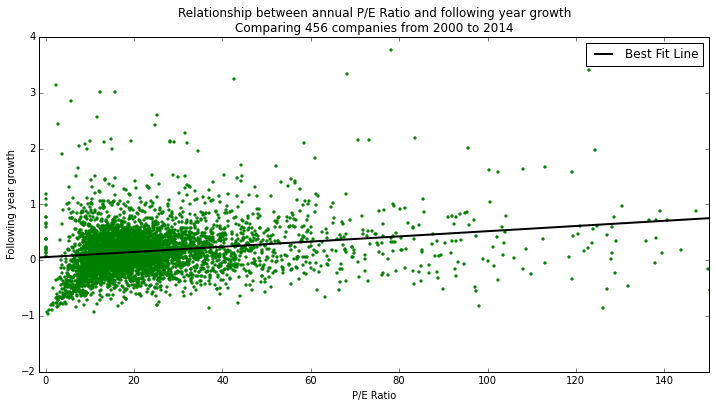
\includegraphics[width=\textwidth]{vis/pe-ratio-abs.png}}
	\label{fig:pe-abs}
\end{figure}

The best fit line was calculated using the standard Least Squares method. If the P/E ratio was indeed predictive, we might have expected a steeper slope in the best fit line, but we can see that there is a very weak correlation at best. It should also be noted that the more we remove outliers, the lower the slope becomes. This indicates that the the line is probably being pulled up by outliers rather than an actual correlation in the data. 

We can investigate the data further using a boxplot. Figure \ref{fig:pe-box} divides companies into two categories. The first category, $Gain\ Companies$, are companies whose share price increased in a given year, and the second category, $Loss\ Companies$, are companies whose share price fell in a given year. The box plot shows the distribution of P/E Ratios for each category.

\begin{figure}[H]
	\caption{Investigation of P/E Ratio predictive value using Box plot}
	\centerline{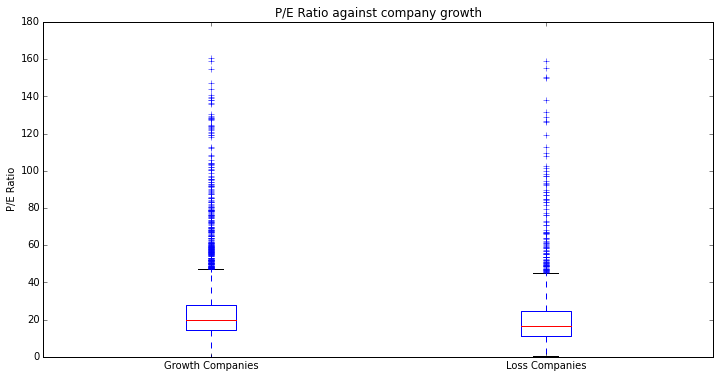
\includegraphics[width=\textwidth]{vis/pe_box.png}}
	\label{fig:pe-box}
\end{figure}

If the P/E Ratio was predictive, we would have expected a noticable difference in the P/E Ratio distribution of companies whose share increased, and those whose share price decreased. However, this is not the case. It is clear that the P/E Ratio distribution between these categories is almost identical. We can therefore conclude that the P/E Ratio has little or no predictive value when it comes to estimating company performance for the following year.

\section{Price to Book Ratio}

The second metric for the value of a company that we will look at is the Price to Book Ratio. The price to Book Ratio is calculated as

\begin{math}
  \\
	\text{P/B Ratio} = \dfrac{\text{Share Price}}{\text{Book Value of Company}}
	\\
\end{math}

Informally, what this calculates is the ratio between the value of a company according to the market and the value of the company on paper. If the ratio is high, this might be a signal that the market has overvalued a company and the price may fall over time. Conversely if the ratio is low, that may signal that the market has undervalued the company and the price may rise over time. We should then expect to see a relationship between high P/B ratio and low returns in the following year. 

To investigate this relationship, we plotted the P/B ratio for of 316 companies on the 31st of December against the change in stock price for the following year. We gathered these data points from the year 2000 to 2014. Figure \ref{fig:pb-abs} is a graph of this relationship.

\begin{figure}[H]
	\caption{Relationship between P/B Ratio and following year growth}
	\centerline{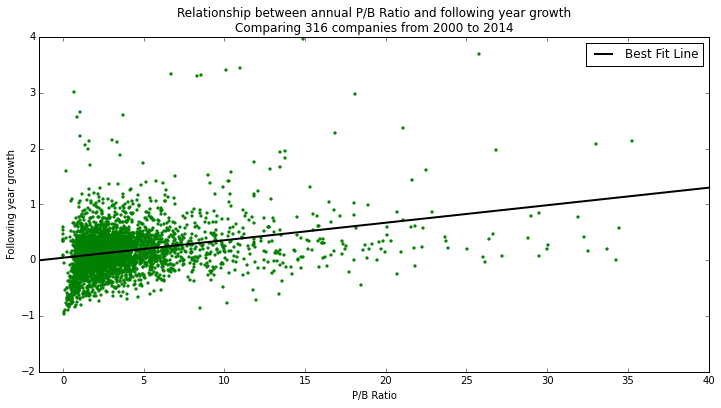
\includegraphics[width=\textwidth]{vis/pb-ratio-abs.png}}
	\label{fig:pb-abs}
\end{figure}

Just as in the P/B diagram, the best fit line was calculated using the standard Least Squares method. Although slope of the best fit line is greater than that of the P/E ratio, this is the opposite of what we might have expected. The data suggests that a high P/B ratio is somewhat  predictive of a high growth in the stock price. This is unexpected result directly opposed to available literature on the subject \cite{jensen1997new}. 

One hypothesis is that a high P/B ratio could be a signal of investor confidence like the P/E Ratio and so we might be able use the argument about how an investor confidence could be a predictor of growth. More likely, we suspect, is that the data used does not control correctly for the expected growth in all companies over the studied time period, from 2000 to 2014. Even accounting for the Great Recession, the stock price of most companies in our dataset did grow from year to year. However, this does not fully explain why the slope of the P/B Ratio best fit line is greater than the slope of the P/E Ratio best fit line. One would have expected at least a lesser slope if the expected slope was an inverse relation. 

To better understand the predictive value of the P/B Ratio we can use a box plot. Figure \ref{fig:pb-box} divides companies into two categories, exactly as in the earlier P/E Ratio example. The box plot shows the distribution of P/B Ratios for each category.

\begin{figure}[H]
	\caption{Investigation of P/B Ratio predictive value using Box plot}
	\centerline{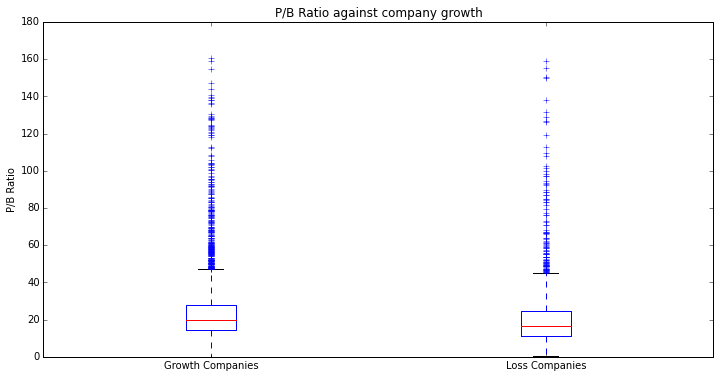
\includegraphics[width=\textwidth]{vis/pb_box.png}}
	\label{fig:pb-box}
\end{figure}

It is evident that this diagram tells a very similar story to the P/E Ratio diagram. We can see that companies that grew and companies that shrank had an almost identical distribution of P/B Ratios. If it were predictive, we would have expected different distributions for each category. We can therefore conclude that the P/B Ratio also has little or no predictive value when it comes to estimating company performance for the following year.

\section{Limitations of Fundamental Analysis}

There is an obvious problem in Fundamental Analysis. We are trying to find the quantify the true value of a company when almost every company has in some way or another some purely qualitative value.

Fundamental Analysis methods do not attempt to capture these qualitative values, and so it difficult to build a software solution to do so. This leaves a large gap in knowledge an algorithm could learn about a company. How should it quantify the value of a brand, the size of its customer base, or a competitive advantage?

These are three examples of some of the many things that a human investor might take into account when deciding who to invest in, but they are untouchable within the scope of this project. 

Instead, we are limited to purely quantitative company metrics. We will look at two of the most common metrics, Price to Earnings ratio and Price to Book ratio.

\section{Fundamental Analysis - Conclusion}

We evaluated two Fundamental Analysis metrics and found no conclusive proof of their predictive value.  

These predictions are also very long term, looking one year into the future. Predictions on this time scale were not the focus of the project. Instead we wanted to focus on predicting daily trends in the market.

Because of these issues that we moved away from Fundamental Analysis.

\chapter{Technical Analysis}


The second approach we take at solving the problem of market prediction is to use Technical Analysis. This approach tries to find recurring patterns and trends within the price of the stock itself.

It should be noted that Technical Analysis goes directly against all forms of the Efficient Market Hypothesis. As explained earlier, even the weak form of the Hypothesis rules out prediction using historic price data alone.

Technical Analysis is used for daily level price prediction which was the original focus of this project. 

tech anal is popular because it is simple and accessable and intuitive

\section{Broad Families of Technical Analysis Models}

If a casual investor was to do some research into trading on the stock market using Technical Analysis they would encounter two broad categories of models. We will demonstrate that one of these is implausible in theory and in practice, while the other although sound in theory, does not work in practice.

\section{Naive Trading patterns}

The first family of technical analysis methods we will look at are those that do not work in theory or in practice. These methods are based on looking for very high level patterns in the stock market price and using these patterns in an attempt to predict the following price movements.

Among the most common of these patterns is the Head and Shoulders pattern, and it is one of the worst offenders of poor methodology in the Technical Analysis of stock market field.

\begin{figure}[H]
	\caption{Head and Shoulders Pattern \cite{website:headshoulders}}
	\centerline{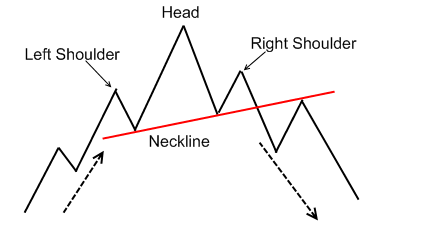
\includegraphics[width=\textwidth]{vis/headshoulders.png}}
	\label{fig:headshoulders}
\end{figure}

Figure \ref{fig:headshoulders} shows a bearish head and shoulders pattern. In this context, bearish is taken to mean falling share prices. The idea is that if a trader sees this pattern, they can expect the market price to then fall. To spot this pattern, a trader is supposed to look for two smaller peaks (the shoulders) surrounding a larger peak (the head). 

However, it can be shown that the pattern does not, and indeed cannot, provide useful information. 

The first issue is that the pattern cannot be identified until after it has happened. Not until the price falls away below the right shoulder, does it become apparent that a head and shoulders pattern has just occured. But this information needed to identify a the head and shoulders pattern is exactly what it was supposed to predict. This leaves no useful information for the trader. If the price were to rise after the right shoulder, it would not be a head and shoulders pattern. A common pattern here is that the investor does not see this as a case where the head and shoulders pattern failed, but instead a case where the head and shoulders pattern didn't exist. This is confirmation bias.

Because of the lack of theorethical support, it is easy to find many additional problems with the head and shoulders pattern. The most obvious one is that because we cannot identify the pattern until after the fact, we can never tell the way the market should move even if the pattern was predictive. Suppose we have observed a series market movements that appear to be similar to those in the diagram up to peak of the right shoulder. We have no way of telling whether the market will continue upwards, or follow the head and shoulders pattern downwards. If the pattern moved upwards when it was supposed to be at the right peak, the right peak could turn out to be a left shoulder of another possible head and shoulders, or even a head peak.

In short, it is impossible to get any useful information from the head and shoulders pattern. However this does not appear to stop investors attempting to use it. A casual investor doing an internet search about trading patterns will more than likely bump into a blog post or an apparently authoritive source telling them how to use this pattern, or one like it, to profit on the market. 

There is no shortage of similar patterns to be found in online literature, but almost all fall into the same problems as the head and shoulders pattern. All information available from these models is only useful in retrospect. 

\section{Moving Average Crossover}

Next, we move to Technical Analysis models that are sound in theory. These models work on a statistical basis rather than patterns and make explicit predictions about the future. One of the simplest and most common models of this type is the Moving Average Crossover strategy.

The moving average crossover strategy relies on the interaction between two moving average calculations. One is a short moving average, and the other is a long moving average. The short moving average might be the mean price for the last 10 days, and the long moving average might be the mean price for the last 20 days for example. When the short moving average crosses under the long, this can be intrepreted as a negative signal that the market is trending downwards. Conversely if the short moving average crosses over the long, this can be intrepreted as a positive signal that the market is trending upwards. The points at where these events happen are called the crossover points and can be categorised into negative and positive crossovers points.

\begin{figure}[H]
	\caption{Moving Average Crossover}
	\centerline{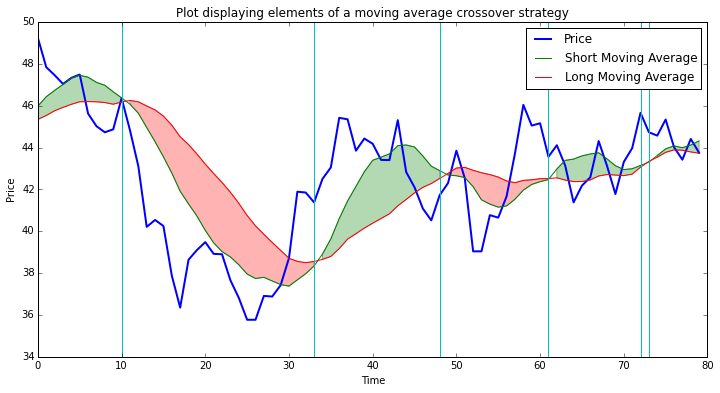
\includegraphics[width=\textwidth]{vis/macrossover.png}}
	\label{fig:macrossover}
\end{figure}

In figure \ref{fig:macrossover}, the red areas are where the short moving average is below the long moving average and the green areas are where the short moving average is above the long moving average. The diagram seems to give us hope for this strategy. The large green and red areas on the left of the diagram do indeed appear to be predictive of market upward and downward trends respectively. 

However, while it is attractive to look at the crossover points on the left of the diagram, one should not ignore the less significant crossover points on the right of the diagram. These are crossover points just as much as the ones on the left area but these are not as predictive for market trends. We need to choose a long and short periods moving average to maximize the predictive value.

\subsection{Evaluating the Moving Average Crossover Model}

To evaluate the predictive value moving average crossover model, we attempted to build a predictor using these crossover signals (negative and positive) as the input features and the market trend for the following day as the dependent variable we are trying to predict. We performed a rigorous evaluation of long and short term pairs on a training set, and tested the winning long/short term pair against an independent test set.

To perform this analysis, we assembled a database of daily prices of all 30 companies in the Dow Jones from the year 2000 to 2014.

This data was then augmented with $49$ new moving average columns. The first of these columns contained the 1-day moving average price, the second contained the 2-day moving average price, etc., up to the 50-day moving average price. This precomputation of the moving averages greatly decreased the time taken to train the model.

The data was split into a training and test set. For simplicity, we divided the data based on company. We chose 20 random companies and used them as the training set. The remaining 10 companies were used as a test set. This is similar to the single-holdout method, which under normal circumstances is not considered to be statistically credible. However there was sufficient data in this case for single-holdout to be viable. There were over 74,000 data points in the training set and over 38,000 in the test set.

The model itself was purposefully kept extremely simple so as to remain true to the intended usage of the moving average strategy. When a positive crossover occurred (short crosses over long), the model predicted the stock price would increase tomorrow, and when a negative crossover occurred it predicted the stock price would fall tomorrow. Deciding which long and short term periods to use can be seen as equivilent to finding the best hyperparameters for the model. This is model selection.

We perform a grid search over all possible long and short period pairs. For each period pair, we find the crossover points between them. For each crossover point, we make a prediction based on its positivity or negativity, and compare tomorrow's predicted trend against the actual trend. We can then calculate the accuracy of this short/long period pair and remember it if it is the best so far.

When we have iterated over all possible long and short pairs, we will have found the best period pair for predicting tomorrow's trend in the training set. Table \ref{table:ma-test-results} displays the top 5 short and long period pairs and their test accuracy.


\begin{center}
    \begin{tabular}{l | l | l | l}
    Rank & Short Period & Long Period & Test set accuracy \\ \hline
    1 & 8 & 35 & 0.5229 \\ \hline
    2 & 8 & 34 & 0.5219 \\ \hline
    3 & 8 & 33 & 0.5127 \\ \hline
    4 & 2 & 37 & 0.5073 \\ \hline
    5 & 2 & 36 & 0.5016 
    \label{table:ma-test-results}
    \end{tabular}
\end{center}

The winning pair after model selection was $8$, and $35$ for the short and long period respectively. We then cross validated this against our test set. Our accuracy on the test set using the $8$, $35$ pair was 0.5157. This is slightly lower than our training score, as should be expected.

We can better understand what the model is doing by looking at the confusion matrix in Figure \ref{fig:ma-confusion}.

\begin{figure}[H]
	\caption{Cross-validation Confusion Matrix for Moving Average Strategy}
	\centerline{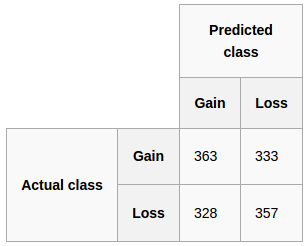
\includegraphics[scale=0.75]{vis/ma_confusion.png}}
	\label{fig:ma-confusion}
\end{figure}

We can now put into context how accurate the model is. We can see a slight increase in the numbers along the principle diagonal, indicating correct predictions. This gives us the slightly better than 0.5 accuracy score. But it is also obvious that the model isn't doing much better than a random predictor. We can quantify this using the Kappa Statistic, which compares the model's performance to a random version of itself based on the confusion matrix. This model scores a kappa of 0.0427, which is not significant. 

We must conclude that the Moving Average Crossover is not predictive in any meaningful way, at least for predicting the movement of companies on the Dow Jones.

\section{Additional Technical Analysis Models}

Although we had no success using moving average crossovers, there are many other technical analysis indicators that are regularly used by traders. We will evulate a further five of the most common indicators. These indicators are described below.

\begin{description}
  \item[Weighted Moving Average] A weighted moving average is the average where later data points are given more weight than earlier data points. In terms of this experiment, the data points will be the prices of individual days. The intuition in using the weighted moving average indicator follows an idea of reverting to the mean, but in this case the mean is calculated using weighted prices. Equation \ref{eq:wma-calc} defines weighted moving average  $wma^{n}_{d}$, on day $d$ using the previous $n$ days.
 
  \begin{figure}[H]
  \begin{center}
      \begin{equation}
        wma^{n}_{d} = \dfrac{n * p_{d} + (n - 1) * p_{d-1} + ... + 1 * p_{d-n}} {n + (n - 1) + ... + 1}
        \label{eq:wma-calc}
      \end{equation}
  \end{center}
  \end{figure} 
    
  \item[Momentum]
  A momentum indictator calculates the relative change in price over the last $n$ days. This is based on a straight forward percentage change. Equation \ref{eq:mom-calc} defines $momentum^{n}_{d}$ which calculates momentum on day $d$ by looking at the price difference from $n$ days ago.
  
  \begin{figure}[H]
  \begin{center}
      \begin{equation}
        momentum^{n}_{d} = \dfrac{p_{d} - p_{d-n}} {p_{d-n}}
        \label{eq:mom-calc}
      \end{equation}
  \end{center}
  \end{figure}  
    
  \item[Bollinger Bands]
  A Bollinger Band indicator calculates the number of standard deviations a price is away from a moving avereage. The intuition is that if the current price is far away from the mean price, then it might signal an upward or downward trend is to follow. Equation \ref{eq:bol-calc} defines $bollinger^{n}_{d}$ where $\mu^{n}_{d}$ is the mean price on day $d$ of the last $n$ days and $\sigma^{n}_{d}$ is the standard deviation in price on day $d$ of the last $n$ days.
  
  \begin{figure}[H]
  \begin{center}
      \begin{equation}
        bollinger^{n}_{d} = \dfrac{p_{d} - \mu^{n}_{d}} {\sigma^{n}_{d}}
        \label{eq:bol-calc}
      \end{equation}
  \end{center}
  \end{figure}  
  
  \item[Relative Strength Index] 
  The Relative Strength Index (RSI) attempts to capture the trading strength of a stock, i.e will how likely a stock price is to continue rising or falling. Borrowing from \citet{wong2003rewarding} for the intuition,
  
  \begin{quotation}
  \textit{Readings of 100 imply that there are pure upward price movements, while readings of 0 imply that there are pure downward price movements. Hence a reading close to 100 indicates an overbought market, while a reading around 0 indicates an oversold market.}
  \end{quotation} 
  
  Much like our other indicators then, RSI should act as an indicator that the market price is about to revert back to a some kind of mean.
  
  Calculation of RSI is done in two parts. First $RS^{n}_{d}$ is calculated. $RS^{n}_{d}$ is, informally, the average price increase over the last $n$ days divided by the average price decrease over the last $n$ days. $RS^{n}_{d}$ is then used to calculate $RSI^{n}_{d}$ which is the relative strength index on day $d$ using the preceding $n$ days.
  
  \begin{figure}[H]
  \begin{center}
      \begin{equation}
        RS^{n}_{d} = \dfrac 
        {\dfrac {1} {n} \sum\limits_{k=d-n}^{d} ( p_{k} - p_{k-1} \mid p_{k} > p_{k-1})} 
        {\dfrac {1} {n} \sum\limits_{k=d-n}^{d} ( p_{k} - p_{k-1} \mid p_{k} < p_{k-1})}  
        \label{eq:rsi-calc}
      \end{equation}
      \begin{equation}
        RSI^{n}_{d} = 100 - \dfrac{100} {1 + RS^{n}_{d}} 
      \end{equation}  
  \end{center}
  \end{figure}  
  
\end{description}

\subsection{Evaluating the Indicators}

In the previous section, when looking at the moving average crossover strategy, we built an extremely simple model that predicted the trend based on a signal. This signal was relatively easy to define, there was a signal when the long and short moving averages crossed over on each other. However with the indicators mentioned above, the definition what constitutes a signal and what doesn't is far more ambiguous. For instance, in regard to the Bollinger Band indicator there is no agreed upon threshold of standard deviation that should signal an upward or downward trend. 

The correct thing to do at this point would be to train many different extremely simple models on many different signal parameters for each indicator, like what was done for the moving averages model. However this would have been extremely computationally expensive. A different approach was required. Instead of generating the signals and using a simple model to predict the following day trend, we used the raw values from the indicators and a more complex model to predict the following day trend. A more complex model should be able to hypothesise what these signals should be, which avoids having to predefine them.

These models will employ machine learning techniques in an attempt to abstract the important signals from our technical analysis indicators. If these models perform well, given the indicator data as input, it must mean that the indicator is indeed useful. If, on the other hand, these models are not successful it probably (but not certainly) means that the indicators are not useful. 

\subsection{Data Preparation}

Before we begin training the models, we must prepare the data to feed them. Because no signals had to be definied, this step was relatively straight forward. 

The primary price database originally prepared in the Data and Tools chapter was used for this experiment. For each company, its price history was iterated over and the value of each indicator for each day was calculated. The results of these calculations were stored in a temporary collection. 

When iteration was completed, the data for each company was standardised so that both high and low priced companies could be used in training and testing the same model. Standardisation shifts and scales the data so that it has a mean of $0$ and a standard deviation of $1$. It should be noted that standardising all of the data in one go, like what is being done in this case, is not correct methodology. Ideally, the training data should be standardised before the test data, and the test data should be standardised using calculations based on the training data. This is done to avoid leakage, when the test data influences the training data. However, this would be difficult to do in this situation as each each company needed to be standardised separately and no division of test and training data has been made yet. Since this error is more likely to artificially increase the models performance than not, and our models will later fail to perform anyway, this error is ignored.

With each the indicator data of each company standardised, the data is stored for later use in testing models. There are 95,407 examples in the database.

\subsection{Error Estimation}

In this step, we determine which class of model should be used on this data. We will compare three types of model, a k-Nearest Neighbors model, a Logistic Regression model, and a Naive Bayes based model. We also need to search a range of hyperparameters for each model. For instance, what value of k do we use in k-NN? To get an error estimation of each model type, we do a grid search over all hyperparameter values and test using nested kFold cross validation. In this case, we split the data into 10 outer folds and 10 inner folds. The inner folds determine the winning hyperparamter which is cross validated by the outer fold. In total, for each hyperparameter there are 100 models trained. Table \ref{table:model-score-indicators} details the models tested, the hyperparameters searched, and their estimated accuracy. 

\begin{center}
  \captionof{table}{Error Estimation Scores}
  
  \begin{tabular}{l | l | l}
	  Model Name & Model Specific Hyperparameters & Estimated Accuracy \\ \hline
	  LogisticRegression & Norm penalization: l1 and l2 & 0.5143 \\ \hline
	  KNeighborsClassifier & k: 5 to 15, weights: uniform and distance & 0.5034 \\ \hline
	  GaussianNB & - & 0.5131
	  \label{table:model-score-indicators}
  \end{tabular}
\end{center}

It is evident from table \ref{table:model-score-indicators} that none of these models were terribly successful. This is a strong sign that the input data, the indicator values, were not predictive of the following day's price trend.

This does not bode well for technical analysis in general. All technical analysis methods that we have tested have failed. However it would seem that our work is supportive of most serious academic literature on the subject. Prominent economist Burton Malkiel summarises the academic attiude towards technical analysis quite well \cite{malkielrandomwalk}.

\begin{quotation}
\textit{Obviously, I am biased against the chartist. This is not only a personal predilection, but a professional one as well. Technical analysis is anathema to, the academic world. We love
to pick on it. Our bullying tactics' are prompted by two considerations: (1) the method is
patently false; and (2) it's easy to pick on. And while it may seem a bit unfair to pick on
such a sorry target, just remember': His your money we are trying to save.}  
\end{quotation}

Whether deserving of it or not, it would be right to analyse what went wrong in the tests that were carried out. Does the fault indeed lie with lack of predictive power in the technical analysis indicators? Perhaps it is that our models were not able to capture their signals.

This question will be answered in the following chapter where we will determine if there is any useful information in the price history at all. Ultimately, we will provide strong evidence that there is in fact no useful information in price history. It logically follows then that any system that tries to leverage price history is doomed to fail. This includes technical analysis models.

\section{Common Problems with Technical Analysis}

For a casual investor, navigating online literature in this area poses a significant challenge. An extremely common theme in this literature is the poor methodology applied to evaluating trading patterns.

We have seen two examples of confirmation bias when we looked at the Head and Shoulders pattern and when we looked at Moving Average crossover points. In the former, patterns that didn't fit the narrative were simply ignored and in the latter people focused too heavily on the instances where it did work.

Even when there is no confirmation bias present, there is very rarely any proper separation of training and test set. Correct methodology would separate these examples so that one could accurately estimate how the model would perform given unseen examples, like it would have to do in the real world. This problem is prevalent when looking for short and long terms in moving average crossover. What many practitioners appear to do is find the best terms for their given time period and expect that to be just as predictive in future periods. This is incorrect methodology. You will always be able to overfit your model to perform well on a single piece of data, but this may not carry over to unseen examples.

Above, we applied the correct methodology. We split the data into test and training sets and determined hyperparameters through cross-validation. This gives us a true estimate of how our best estimator carries over to future data. This proper methodology is not common in online literature.

\section{Technical Analysis - Conclusion}

It might have been expected, that given the popularity of Technical Analysis for stock market trading, that there would have been a more positive result. However, somewhat surprisingly, the data shows that there is little predictive value to be found in Technical Analysis. 

\chapter{Attacking the problem - Machine Learning}

Our final approach to attacking the problem of stock market prediction is to look at machine learning. With machine learning, we will be building models that teach themselves what to look for, and learn to exploit relationships within the data that we might have otherwise missed using Fundamental Analysis or Technical Analysis.

\clearpage
\section{Preceeding 5 day prices}

In Technical Analysis, we attempted to find patterns and trends in the data that we could use to predict the price movement, the trend, for the following day. Ultimately technical analysis failed to produce any notable results, but perhaps it was because the models are not complex enough to capture any hypothetical pattern that might exist in market data.

Similarly to Technical Aanalysis, in this section we will try to apply machine learning techniques to the price of the stock itself. Again, the Efficient Market Hypothesis says that it should not be possible to gain any predictive value from the price alone, but we might be waiting a while for economists to prove that concretely.

The data that we'll we using is the percentage change in closing price of the stock from the preceding 5 days. The dependent variable will be the trend of the 6th day, i.e will the stock price move up or down.

\begin{center}
  \captionof{table}{Data Extract}
    \begin{tabular}{l | l | l | l | l | l | l | l}
	& day0 & day1 &	day2 & day3 & day4 & outcome & outcome-class \\ \hline
0	& 0.0492 &	-0.0029 &	0.0176 &	0.0115 &	0.0028 &	-0.0142 &	0\\ \hline
1	& -0.0029 &	0.0176 &	0.0115 &	0.0028 & -0.0142 &	-0.0028 &	0\\ \hline
2	& 0.0176 &	0.0115 &	0.0028 &	-0.0142 & -0.0028 &	0.0115 &	1\\ \hline
3	& 0.0115 &	0.0028 &	-0.0142 &	-0.0028 &	0.0115 &	-0.0229 &	0

    \label{table:data-example-1}
    \end{tabular}
\end{center}

Table \ref{table:data-example-1} is extract of the first 4 rows in the dataset. Columns labeled day0 to day4 are the percentage change in closing price of the preceding 5 days. We will use the outcome-class as the dependent variable. This column has three classes; $0$ represents a drop in the price, $1$ represents an increase in the price, and $2$ represents no change. This third class is rare, and is ignored for the remainder of the discussion. The dataset that we gathered contained 206635 examples. It was gathered from the the daily closing price of companies in the Dow Jones from the year 2000 to 2014. Before feeding the data into the models as discussed later, it the data rows were randomly permuted to remove and bias the model could learn from an ordered dataset.

\subsection{Error Estimation}

After we have gathered the data, the next step in building our model is choosing which base model we should work with. This step is called Error Estimation. It involves training and testing the performance a couple of different models on the dataset to see which one we should focus on optimizing.

We tested each model by doing a nested kFold test. In this case, we split the data into 10 outer folds and 10 inner folds. The inner folds determine the winning hyperparamter which is cross validated by the outer fold. In total, for each hyperparameter there are 100 models trained.

\begin{center}
  \captionof{table}{Error Estimation Scores}
  
  \begin{tabular}{l | l | l}
	  Model Name & Hyperparameters Tested & Nested KFold Accuracy \\ \hline
	  LogisticRegression & Norm penalization: l1 and l2 & 0.5343 \\ \hline
	  KNeighborsClassifier & k: 1 to 10, weights: uniform and distance & 0.5172 \\ \hline
	  GaussianNB & - & 0.5292
	  \label{table:model-score}
  \end{tabular}
\end{center}

Table \ref{table:model-score} shows the accuracy scores of each model that we tried on the given data. A support vector mechine based model was also tried, but it proved too slow to train with the computational resources at hand. However in smaller trials the SVM model did not seem to be significantly better than any of the model types presented above.

It is immediately clear that there is a problem here. None of the models that we tried got significantly above 0.5\% accurate in our classification test. A coin toss predicting the outcome of the dependent variable would perform similarly to what these models did. Although some models appear to be slightly better, we cannot place too much value in the actual value cross validation score we got here. The nest kFold method does not give us the true accuracy of the model, it only gives us an estimate which should be good enough to choose which model we carry forward to Model Selection. Differences of 1\% or 2\% at this point are not significant. We conclude that none of these models will work at predicting the the trend on the 6th day given the trends of the previous 5 days.

\subsection{Analysis of Model Failure}


The failure of all models there were tested gives us a strong indication that something is deeply wrong somewhere. In this section, we will show that there is good evidence that the problem is in fact that there is no information to be found from the previous 5 day prices. This is, of course, exactly what the Efficient Market Hypothesis predicts.

\subsubsection{Model Complexity}

It is important here to clarify what we mean by model complexity. The complexity of a model is the size of the set of hypothesis that it can produce. A hypothesis is a guess that the model can make about the relationship between input features and the dependent variable. A linear model would guess, or hypothesize, that the relationship is a linear combination of the input features. A nearest neighbours model would guess that the relationship is going to copy previously seen examples. A model that can produce a larger number of hypothesis is more complex than one which can produce a smaller set. It is also important to note that these hypothesis sets do not necessarily overlap. One model may be more complex than the other, but that is not to say that the best hypothesis does not belong to the model of lesser complexity.

One possible reason for the failure of our models in the previous section is that the models we tried were not sufficiently complex. However, the models and hyperparameters that were tested covered a very large hypothesis base. If there was a good hypothesis to find, it is reasonably that one of the models should at least have been better than a coin toss at predicting the trend. 

We can also inspect the effect of model complexity visually using graphs. For convenience we choose to model the kNN model here. Analysis of the kNN model is simplier and no less consequential than the other models.

The complexity of kNN can be varied by changing k, where k is the number of neighbours the model will consider to make its prediction. A low value of k means the model will look at only a few of the closest neighbours to attempt to infer the value of the input, and conversely a high value of k means that the model will consider a larger number of neighbours. Recall that our measure of complexity is the size of the hypothesis set. It follows that the complexity of kNN is inversely proportional to k. Given $n$ examples, a uniformly weighted 1-NN model is able to produce $n$ hypotheses, but a $n-NN$ model can only produce one hypothesis.

\begin{figure}[H]
	\caption{kNN Validation Curve}
	\centerline{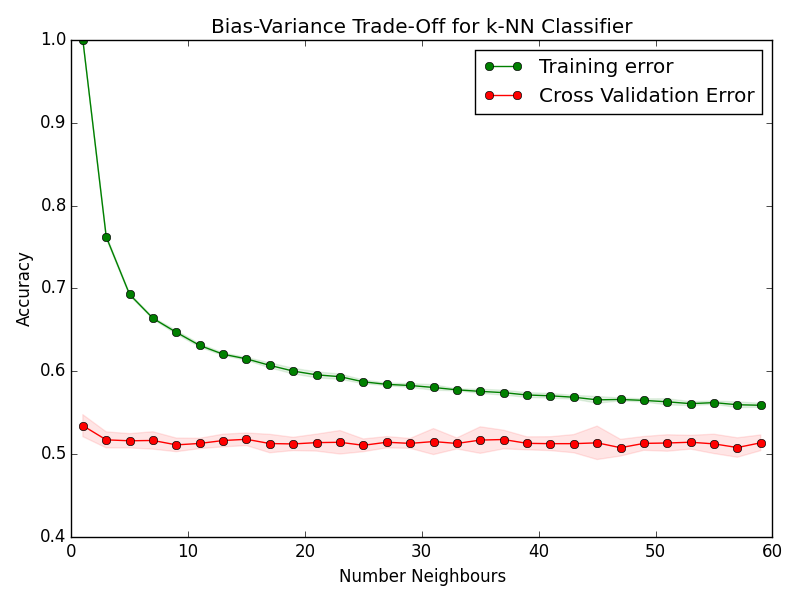
\includegraphics[scale=0.5]{vis/prices-bias-variance.png}}
	\label{fig:knn-validation}
\end{figure}

Figure \ref{fig:knn-validation} plots the validation curve for the kNN model. To generate this graph, we generated 60 kNN models with different k values. The training and test error for each value of k was then plotted. Since the complexity of the model varys with k as explained above, we can interpret the graph as being a performance comparison of models of varying complexity. Normally in such a graph we would expect the training and test errors to converge, but this is clearly not happening for this graph. No matter what the complexity of the model, the Cross Validation Accuracy never rises significantly above 0.5\%. We can then conclude that the problem is not due to the complexity of the model.

\subsubsection{Training Data}

If the problem does not lie with the complexity of our models, then maybe the problem is due to the amount of training data that we have. Perhaps if we had more data, we could build better models.

As mentioned previously, the dataset we used for training and testing these models had over 200,000 examples. This seems like it should be enough, but maybe the stock markets are so complex they need more.

To properly diagnose this, we can plot the learning curve. In the Validation Curve, we varied the complexity of the model. In the Learning Curve, we will vary the number of examples presented to the model. Because of computational resources available, we were forced to constrain the number of examples in the Learning Curve to approximately 15,000. This is much smaller than the 200,000 examples in the dataset, but certainly not too small to ignore the findings.

\begin{figure}[H]
	\caption{kNN Learning Curve}
	\centerline{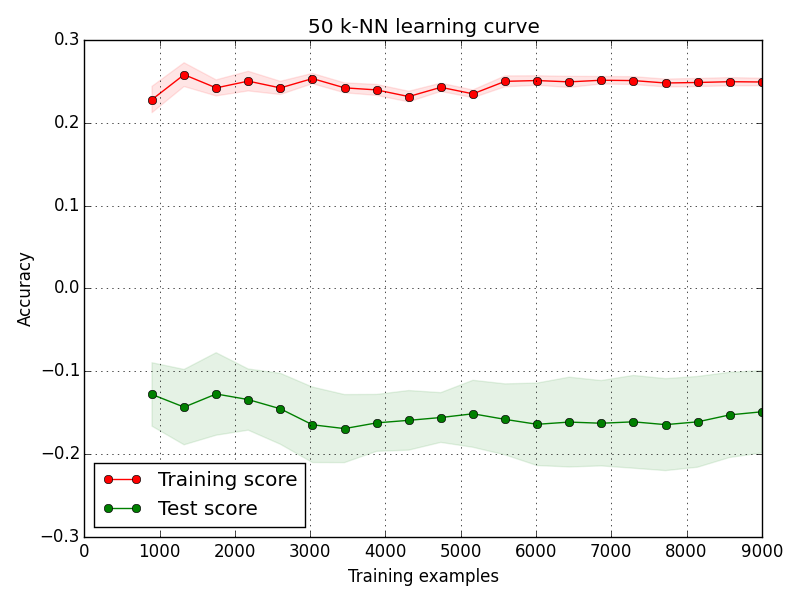
\includegraphics[scale=0.75]{vis/50-learning-curve-15000.png}}
	\label{fig:knn-learning}
\end{figure}

Figure \ref{fig:knn-learning} shows the effect of varying the number of examples on the model. Normally in a Learning Curve graph, you would expect the test and training errors to converge. The intuition is that as the model is presented with more data, it is better equiped to come up with better, more general, hypotheses. Because these improved hypotheses are more general we expect the training accuracy to decrease (less overfitting), but the test accuracy to increase (less underfitting). However we can see that this is not the case for our graph. The graph shows that for our model, the test and training accuracy remain apart and do not begin to converge no matter how much data they were given. We can then conclude that the problem is not due to lack of data for training and testing our model.

\subsection{Preceeding 5 day prices - Conclusion}

In this section, we attempted to train a model to predict the trend in the 6th day given the trends of the previous 5 days but all models were unsuccessful. We then analysed why they might have failed and concluded that it was a problem with neither the complexity of the models nor the amount of data we had to train the models.

We must then conclude the the problem must lie in the data itself. It would seem that the preceeding 5 day trends contain no information useful in predicting the following day trend. This supports our findings in the Technical Analysis approach and the Efficient Market Hypothesis.

Clearly we must begin to look at using external data.

\clearpage
\section{Related Assets}

With the failure of using the price itself to predict stock movements, we turn to other sources of predictive value. Prehaps the most obvious source we should seek to use is the movement of assets related to the Dow Jones.

Intuitive, one might suppose that when the price of Oil rises, that is a good sign for the Dow Jones and we can expect it to rise too. Similarly, if the price of Oil falls we might expect the price of the Dow Jones to fall with it. In this section, we will search for features that rise and fall with the Dow Jones index.

\subsection{Data}

Since in the last section we showed that yesterdays prices appear to have no influence on todays prices, it is unreasonable to expect yesterday's prices of related assets to influence today's Dow Jones price. Because of this, instead of predicting based on yesterday's prices, we will predict based on price movements in assets that are traded earlier in the day than the Dow Jones. For example, we will will use the price movements of assets that are traded in Europe and Asia to predict the trend in the Dow Jones, which is traded in New York. If markets in Europe and Asia as trending heavily in one directly, it might follow that the Dow Jones will also trend that way when the markets open. What is important is that in the real world, we can observe the trends of our related assets before we need to make a prediction of our the trend in the Dow Jones.

However, some market times overlap. For instance, the London Stock Exchange and the New York Stock Exchange are both trading at the same time for approximately 4 hours daily. It would be ideal then to have price data then which we can cleanly partition into intraday prices before and after the Dow Jones begins. However, this data is not easily available in the public domain. Intraday price data is a commodity and not something which is distributed as freely as interday price data. Quandl, which has been our source of much of the data up to this point, does not offer intraday price data.

We are then forced to accept subpar data which does not allow for proper preparation. We will continue to use the data provided by Quandl from which we can extract the daily closing price of each asset and index. This is opening us to problems of leakage, where the test set can influence the training set. It is concievable that the trend in the New York Stock Exchange can effect the trend in the London Stock Exchange, even though it only opens in the final 4 trading hours. Due to this issue we must be cautious and suspecious positive results moving forward. It is unfortunate that later in the report, when we implent the trading algorithms in Quantopian, we will show that positive results mentioned in this section do indeed appear to be because of this error in the data.

Temporaraly ignoring the aforementioned issues, we gathered data for 8 features from Quandl. These features are detailed below.

\begin{description}
  \item[DAX] The German DAX index is essentially equivilent to the Dow Jones except that its components are 30 major German companies traded on the Frankfurt Stock Exchange.
  
  \item[DAX FUT] We also considered DAX futures. Futures are a stock market derivative product.
  
  \item[FTSE] Similar to the Dow Jones and the German DAX. Traded on the London Stock exchange, its components are a selection of 100 large UK based companies. Commonly known as the FTSE100
  
  \item[N225] The Nikkei 225 has 225 large Japanese companies as components as is traded on the Tokyo Stock Exchange.
  
  \item[SSE] The SSE Composite Index is an index covering all stocks that are traded on Shanghai Stock Exchange. It is itself traded on the Shanghai Stock Exchange.
  
  \item[AUD] The Australian Dollar to US Dollar exchange rate
  
  \item[EUR] The Euro to US Dollar exchange rate
  
  \item[OIL] Brent Crude Oil futures prices
      
\end{description}

A decision was made to use the price of the Dow Jones index rather than the price of the components, or companies, themselves as the dependent variable. This was due to the fact that the features listed above are not specific to any one company, although it could be argued that some features might influence some companies more than others. Determining the predictive value for each feature for each company would have made modeling significantly the problem more complex and computationally time consuming. For simplicity, the price of the Dow Jones index was used as the dependent variable in this section.

\subsection{Exploration of Feature Utility}

The next step in creating a model to predict the daily trend of the Dow Jones Index is to determine the predictive value of the features. To do this in an exploratory and qualitative manner, we first analysed the predictive value of each feature on its own. We trained 8 models, one for every feature. Each of these models used exactly one of the features to try and predict the trend for the Dow Jones Index. For each feature a, kNN model was trained and cross validated. Figure \ref{fig:single_feature_prediction} shows the cross validation results for each feature.

\begin{figure}[H]
	\caption{Single Feature Prediction Results}
	\centerline{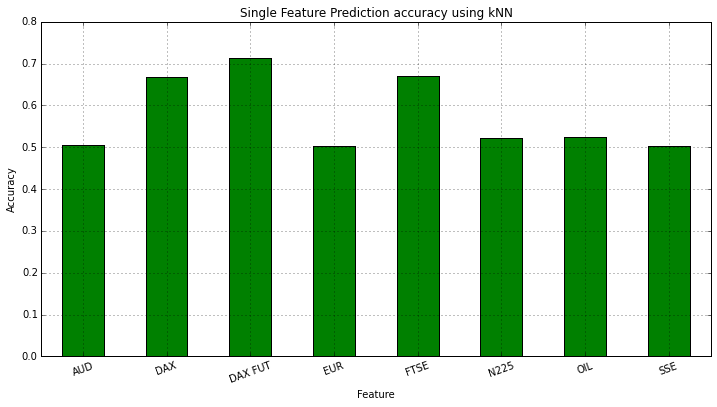
\includegraphics[scale=0.5]{vis/single_feature_prediction.png}}
	\label{fig:single_feature_prediction}
\end{figure}

It is evident from the graph that there is indeed some predictive value in this dataset. There are three features that appear to be highly predictive. The German DAX, DAX futures, and the FTSE100 are all roughly 70\% accurate without doing any work whatsoever.

\subsection{Modeling}

Now that we know that there is at least some predictive value in our dataset, we can begin to create our model.

\subsubsection{Error Estimation}

Similar to what we attempt to do with the model based on the historical prices, the first step in creating our model is error estimation. In this step we estimate the performance of various classes of model.

We used a nested kFold method to perform the error estimation. The inner kFold performed a Grid Search over a set of hyperparameters.  The outer kFold was responsible for the cross validation of the set of hyperparameters found within the inner kFold. The Grid Search searched over two domains. The first domain was the hyperparameter determining how many of the $k$ best features to keep. For instance, the search might determine that it was best to keep the top 3 most predictive features. The second domain were the hyperparameter specific to the model being tested. Table \ref{table:asset-error-est} details the model class tested, the model specific hyperparamters searched over, and the cross validation score.

\begin{center}
  \captionof{table}{Error Estimation Scores}
  
  \begin{tabular}{l | l | l}
	  \textbf{Model Name} & \textbf{Model Specifc Hyperparameters} & \textbf{Estimated Accuracy} \\ \hline
	  LogisticRegression & Norm penalization: l1, l2 & 0.5717 \\ \hline
	  KNeighborsClassifier & $0 < k \leq 25$, weights: uniform, distance & 0.7251 \\ \hline
	  GaussianNB & - & 0.7208
	  \label{table:asset-error-est}
  \end{tabular}
\end{center}

The scores from table \ref{table:asset-error-est} look hopeful. We can see that the kNN model has the best estimated accuracy, albeit not by much. This means that this is the model we should bring forward to Model Selection to further optimise it.

\subsubsection{Model Selection}

Now that we have our winning model class, kNN, we now need to estimate the optimum hyperparameters for our model. 

A kNN model has two important hyperparameters, $k$ and how to weigh examples in the neighborhood. $k$ dictates how many neighbors the model should examine to make a prediction. We can then weigh those neighbors either uniformly or by their distance to our input. We can search over the same value space as we did in Error Estimation for kNN, $0 < k \leq 25$ and weights $uniform$ or $distance$. We will also be searching for the best number of features to keep in the model, this can be treated as another hyperparameter.

After performing a grid search over the value space and cross validating each combination of hyperparameters, we find that the best combination of hyperparameters gives us a cross validated accuracy of 74.63\% at predicting Dow Jones Index daily trends. Table \ref{table:asset-model-sel} shows the best combination of hyperparameters found.

\begin{center}
  \captionof{table}{Model Selection Results}
  
  \begin{tabular}{l | l}
	  \textbf{Hyperparameter} & \textbf{Best value} \\ \hline
	  Number of features to keep & 3 \\ \hline
	  Number of nighbours to examine & 14 \\ \hline
    Method of weighing neighbours & uniform
	  \label{table:asset-model-sel}
  \end{tabular}
\end{center}

Table \ref{table:asset-model-sel} indicates that the search determined that keeping only three of the original 8 features gave us the best cross validation score. This is in line with what we might have expected from the exploration of the predictive value of the features where we pointed out three features that appeared to be were highly predictive already.

By training the model on the full dataset with the winning hyperparameters and inspecting the 3 features the feature selector decided to keep, we can see that they are indeed the three features we assumed would be predicted. The German DAX, DAX futures, and the FTSE100 are the features selected in the final model.

\subsection{Related Assets - Conclusion}

In this section we gathered data for 8 features that could conceivably have some predictive value for the Dow Jones. We explored the predictive value of each feature visually to gain some sense of the data and then followed the precisely correct methodology to end up with an optimal model. The final model had an estimated accuracy of 74.63\%, which is significant for stock market data.

However, as warned by the data section, we should be cautious of such high accuracy figures. Due to lack of publicly available intraday price data, we might have some leakage of the test set that is skewing our result. Later in the report, when we try to translate this model to a trading simulation,  We will demonstrate that this error is most likely what is giving such a high accuracy score and that it would not work as well in the real world. 

\clearpage
\section{Analyst Opinions}

With the apparent success of using related assets to predict daily movements in the Dow Jones, we continue our search for additional predictive features. In this section we will attempt to use analyst opinions to predict the same day trend.

An analyst opinion is a prediction of a particular research firm on a particular stock. For instance, a large investment research firm such as JP Morgan might issue an opinion on Intel stock. They may upgrade or downgrade their estimates of stock performance, may recommend buying or selling the stock at the current price.

It would seem intuitive that these recommendations should be predictive. There are two reasons why that might be true. The first reason that these recommendations might truely be predictive of the price. One can imagine that large research firms such as JP Morgan would employ skilled analysts that are able to make accurate predictions. The second reason is less optimistic and assumes that these predictions are self-fulfilling prophecies. If multiple large investment firms upgrade or downgrade their opinion of a stock on the same day, it is certainly concievable that the opinions themselves are enough to shift the market regardless of their true predictive value.

However, it should not matter to us why they are predictive. For whatever reason, if these opinions can predictive we should be able to build a model to utilise them.

\subsection{Data}

Conveniently, Yahoo Finance provides an open database of opinions issued by large research firms. The database covers all major stocks including the components of the Dow Jones, the 30 companies of interest to the project. 

One small difficulty in obtaining this data is that it is provided in a HTML table on the Yahoo Finance website. This means that it was not directly downloadable as a csv file or an equivilent easy to use file format. Because of this, a small web scraper had to be constructed. 

The web scraper was constructed in python. The scraper began by sending 30 HTTP get requests to Yahoo Finance, one for each company. The responses were then parsed using the BeautifulSoup4 HTML parsing library. After the HTML was parsed it was trivial to extract the data in a more usable format. The extracted data for all companies was cached in a single CSV file. In total, 3584 analyst opinions were gathered from the year 2000 to 2014.

\begin{center}
  \captionof{table}{Analyst Opinion Data}
  
  \begin{tabular}{l | l | l | l | l | l}
\textbf{Date}        & \textbf{Research Firm}      & \textbf{Action}       & \textit{From}         & \textbf{To}                   & \textbf{Symbol} \\ \hline
2001-04-25  & First Union Sec    & Downgrade    & Strong Buy   & Buy                  & CSCO \\ \hline
2001-04-25  & AG Edwards         & Downgrade    & Accumulate   & Maintain Position    & VZ \\ \hline
2001-05-01  & Salomon Smth Brny  & Upgrade      & Neutral      & Outperform           & PG \\ \hline
2001-05-07  & Prudential         & Downgrade    & Hold         & Sell                 & JPM \\ \hline
2001-05-08  & Mrgn Stnly         & Upgrade      & Neutral      & Outperform           & CSCO
	  \label{table:opinions-data}
  \end{tabular}
\end{center}

Table \ref{table:opinions-data} Displays what the gathered data looks like.

It should be noted that in this section we will be trying to predict the daily movement of individual companies prices rather than the Dow Jones index as a whole as we did in the last section. This is because each opinion very explicitly relates to a single company.

Also note that these opinions are almost always issued before the market opens. It is therefore acceptable to use these opinions to predict the movement on the market for that day.

\subsection{Data Exploration}

As we did in the previous section, to get a better sense of our data we will explore it a little further.

The company with the most opinions in the gathered dataset is Intel (INTC) which 326 individual analyst opinions. To get a sense of whether the data might be useful, we can plot these opinions in relation to the INTC price.

First we filtered the dataset so that we only consider INTC opinions. We then aggregated the opinions that were issued on the same day by counting the number of Upgrades and Downgrades. Finally, the aggregated opinions were merged with the INTC stock price. This data was then plotted.

\begin{figure}[H]
	\caption{Visualisation of analyst opinions and INTC price}
	\centerline{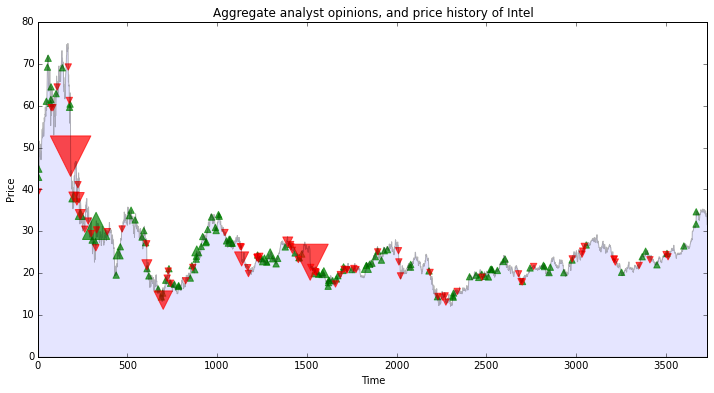
\includegraphics[scale=0.5]{vis/analyst_opinions.png}}
	\label{fig:opinions_vis}
\end{figure} 

Figure \ref{fig:opinions_vis} visualises the relationship between opinion sentiment (Upgrade or Downgrade) and price. Green upwards pointing triangles signal an upgrade and red downwards pointing triangles signal a downgrade. The size of the triangle represents the number of coinciding opinions across all research firms. For instance the large red down pointing triangle on the left hand side of the diagrm is a point representing 9 separate research firms all downgrading their opinion of INTC on the same day.

From visual inspection it would appear there may indeed be some value in these opinions, but we cannot be certain until we attempt to build a model.

\subsection{Data Preparation}

As evident from Table \ref{table:opinions-data} all of the feature values in the dataset are labels and categories, not numerical data. This presents a problem. The machine learning library used in this problem, sklearn, does not provide models which can handle non-numeric data. We must therefore transform our data into numeric form.

The correct way to transform a label type feature is to use One-hot Encoding. One-hot Encoding will transform a single feature with $n$ unique values into $n$ different features with binary values.

\begin{figure}[H]
\caption{One-hot Encoding Example}
\subfigure[Before]{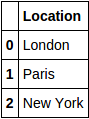
\includegraphics[scale=0.6]{vis/before_encoding.png}}
\hfill
\subfigure[After]{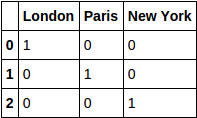
\includegraphics[scale=0.6]{vis/after_encoding.png}}
\label{fig:one-hot}
\end{figure}

Figure \ref{fig:one-hot} demonstrates the concept of One-hot encoding. After One-hot encoding, the original feature is removed but no information is lost. To signify a value in the original column, a $1$ is placed in the new corresponding column.

For the opinions dataset, it was decided that the most important original features are $Research\ Firm$, $Action$, and $To$. $Research\ Firm$ might be important because an opinion from some firms may have more of an influence on the movement than others. The $Action$ column is intuitively important because it summarises the sentiment of the opinion into Upgrade or Downgrade. The $To$ column is the recommendation of the Research Firm, this is also intuitively important because it could be a recommendation to Buy or Sell.

It was then necessary to One-hot encode each of these three features features. This resulted in a total of 266 new feature columns, one new column for each unique value in the original three columns. Now that all the features have been one hot encoded, we can aggregate rows where more than one research firm issued an opinion for the same company on the same date. We will use a sum operation to aggregate the rows accross all columns. For example, if both research firms upgraded a company on the same day then we will merge these rows and place a value of $2$ in the upgrade column.

The entire data preparation stage can be done very concisely a using the Pandas python library.

\begin{lstlisting}[frame=single, caption=Data Preparation Using Pandas]
dataset = pd.merge(opinions,prices,on=['Date', 'Symbol'])

X = dataset[['Date', 'Symbol']] \
    .join(pd.get_dummies(dataset['Research Firm'])) \
    .join(pd.get_dummies(dataset['Action'])) \
    .join(pd.get_dummies(dataset['To'])) \
    .groupby(['Date', 'Symbol']).sum() 
    
y = [frame['Trend'].values[0] for index, frame in \
         dataset.groupby(['Date', 'Symbol'])]
\end{lstlisting}

\subsection{Error Estimation}

With our data prepared, we must decide which class of model to use.

We used a nested kFold method to perform the error estimation. The inner kFold performed a Grid Search over a set of hyperparameters.  The outer kFold was responsible for the cross validation of the set of hyperparameters found within the inner kFold. The Grid Search searched over two domains. The first domain was the hyperparameter determining how many of the $k$ best features to keep. The second domain were the hyperparameter specific to the model being tested. Table \ref{table:opinions-error-est} details the model class tested, the model specific hyperparamters searched over, and the cross validation score.

\begin{center}
  \captionof{table}{Error Estimation Scores}
  
  \begin{tabular}{l | l | l}
	  \textbf{Model Name} & \textbf{Model Specifc Hyperparameters} & \textbf{Estimated Accuracy} \\ \hline
	  LogisticRegression & Norm penalization: l1, l2 & 0.6627 \\ \hline
	  KNeighborsClassifier & $0 < k \leq 20$, weights: uniform, distance & 0.6564 \\ \hline
	  MultinomialNB & - & 0.6729
	  \label{table:opinions-error-est}
  \end{tabular}
\end{center}

The scores from table \ref{table:opinions-error-est} look positive. We can see that the MultinomialNB model has the best estimated accuracy. This means that this is the model we should bring forward to Model Selection.

\subsection{Model Selection}

MultinomialNB being the model that won in the Error Estimation round, it should now be the model that we focus on in Model Selection. 

The MultinomialNB model is a naive bayes classifier and only has one hyperparameter. The hyperparameter, called alpha in sklearn, controls the additive smoothing in the model. What exactly additive smoothing is is out of the scope of this report, but all we need to know is that it is a hyperparameter that should be searched over to optimise the model. 

At the same time as we are searching over the model hyperparameter, we will again be searching for the best $k$ features to keep.

\begin{center}
  \captionof{table}{Model Selection Results}  
  \begin{tabular}{l | l}
	  \textbf{Hyperparameter} & \textbf{Best value} \\ \hline
	  Number of features to keep & 11 \\ \hline
	  MultinomialNB alpha & 0.7333
	  \label{table:opinions-model-sel}
  \end{tabular}
\end{center}

Table \ref{table:opinions-model-sel} shows the best set of hyperparameters found in the search. The winning model had a cross validation accuracy of 67.40\%.

\subsection{Analyst Opinions - Conclusion}

In this section we gathered a list of analyst opinions and used them to build a model to predict the same day price movement for companies in the Dow Jones. Although concise in its final version, the data preparation for this section proved difficult to get right. The final model had an estimated accuracy of 67.40\% which is an extremely positive result. 

Although the data used in this section does not have the leakage problems the data in the last section had, we will unfortunately see that we cannot profitably trade on the stock market using this model either. 

\clearpage
\section{Disasters}

The final source of predictive data we will consider are natural disasters in the United States. 

It is easy to see why these might be predictive of changes in the stock price. A large storm, for instance, could damages some of the company's machinery or interfere with manufacture and logistics. In turn, this could have an impact on the company's profit and therefore their stock price.

\subsection{Data Preparation}

The first task was to gather a database of natural disasters in the United States. This data is provided by EM-DAT, The Internation Disaster Database \cite{disasterdb}. Disasters in this dataset are gauranteed to be relatively large. The website states the qualifications necessary for a disaster to be entered into the database

\begin{quotation}
\textit{In order for a disaster to be entered into the database at least one of the following criteria has to be fulfilled:}
\begin{itemize}
  \item \textit{10 or more people reported killed}
  \item \textit{100 people reported affected}
  \item \textit{a call for international assistance}
  \item \textit{declaration of a state of emergency}
\end{itemize}
\end{quotation}

 All disasters occuring in the United States from the year 2000 to 2014 were extracted. Before any further preparation, there were 423 entries in this dataset.

Disasters with missing or invalid dates were then removed. Following this, disasters with anomalous durations were removed. Figure \ref{fig:disaster-data} shows that there were three clear outliers in this regard. These were removed from the dataset. After all preparation was completed on this dataset, there were 395 disaster events remaining.

\begin{figure}[H]
	\caption{Anomolies in the disaster data}
	\centerline{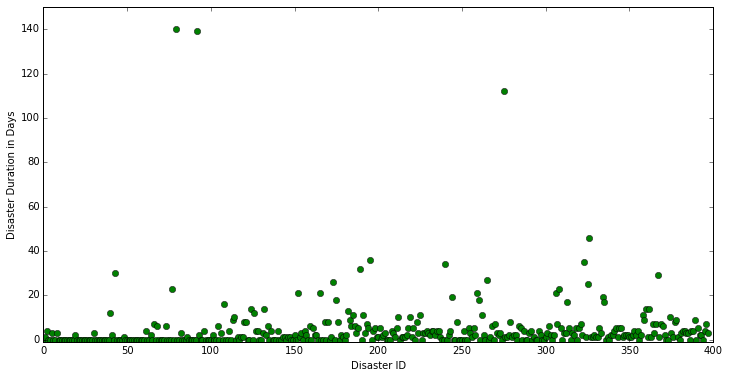
\includegraphics[width=\textwidth]{vis/disaster_data.png}}
	\label{fig:disaster-data}
\end{figure}

Similarly to the Related Assets section, this data does not relate specifically to any one company. Because of this, we will look at price changes of the Dow Jones index, rather than any of its component companies. 

\subsection{Predictive Value of Disasters}

We will first determine the predictive value of the disaster events. The goal of this experiment is to decide whether the price movements of the Dow Jones during disaster times are any different to non-disaster times. If disasters contain any predictive value, positive or negative, we should be able to observe a difference in market behaviour during disaster times.

For each disaster, we determined how much the Dow Jones price index moved in the duration of the disaster. Equation \ref{eq:disaster-calc} shows how this was calculated where $P_{start - 1}$ is price of the Dow Jones the day the before the disaster began and $P_{end}$ is the price of the Dow Jones the day the disaster ended. The varying length of disasters is controlled for by diving by the change in price by the length of the disaster. This equates to an average price movement for each day of the disaster. 

\begin{figure}[H]
\begin{center}
    \begin{equation}
      \text{Disaster price change} = \dfrac{p_{(end)} - p_{(start - 1)}} {p_{(start - 1)}} * \dfrac{1}{Disaster Duration}
      \label{eq:disaster-calc}
    \end{equation}
\end{center}
\end{figure}

Next, daily prices changes in the Dow Jones were calculated for days where no disaster was occuring. Because disaster duration is controlled for, this allows the disaster price changes to be directly compared to daily expected price movements in the Dow Jones.

At this point we have two independent, but comparible, datasets. One contains average daily price movements of the Dow Jones in times of Disaster. The other contains daily price movements of the Dow Jones in times of no Disaster. 

To visualise these datasets, figure \ref{fig:disaster-box} shows a boxplot of their distributions. From visual inspection, we can see immiediately that the data is probably not useful for prediction. If it were useful, we would expect to see a difference in their distibutions.

\begin{figure}[H]
	\caption{Disaster and no disaster price change distributions}
	\centerline{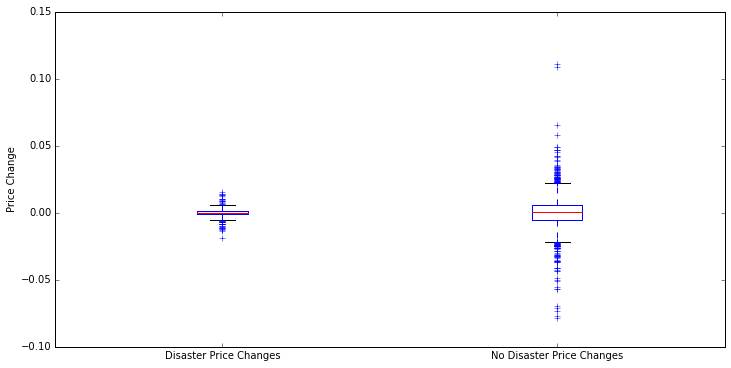
\includegraphics[width=\textwidth]{vis/disaster_box.png}}
	\label{fig:disaster-box}
\end{figure}

To quantify this, we perform a t-test. This results in a t-value of -0.4783 and a two-tailed p-value of 0.6324. Because the p-value is large, we cannot rule out the null hypothesis, that any difference in the distribution of disaster time price movements and non disaster time price movements is due to random chance.

Because there is no significant difference between these two datasets, we will not be able to use disasters to predict price movements in the Dow Jones.

\subsection{Disasters - Conclusion}

Failing to find any predicted value in disasters might be expected in hindsight for three reasons.

\begin{enumerate}
  \item Although all companies are traded on the New York Stock Exchange and have headquarters located in the United States, they are all very much multinational corporations. Multinational corporations are unlikely to be substantially impacted by any single disaster. One top of this, if there are any set of companies that are in a position to mitigate themselves from any disaster they might forcast, it is probably these companies, all of which are among the largest in the world.
  
  \item The second reason that these companies might be uneffected is that they are companies which are largely divorced from whether conditions. It is hard to imagine that companies such as Microsoft, Visa, or Walt Disney are terribly concerned about extreme weather conditions.
  
  \item Finally, it is possible that we simply did not have enough data to begin with. After preparation we had 395 examples spanning 14 years. Perhaps with more data we could target disasters by type or location to specific companies rather than the Dow Jones index as a whole. It is easy to imagine this might have more predictive value.
  
\end{enumerate}

\chapter{Quantopian}

\chapter{Conclusion}

\bibliography{report2}
\bibliographystyle{plainnat}

\end{document}
